\chapter{Two-State Mixing}
\label{appendix:two-state}

In the work of Casten \cite{casten2000nuclear}, an analytical approach is given for the mixing of two different states (energy levels). It starts from the basic idea of two initial levels, each with its corresponding energy $E_1$ and $E_2$, and their associated wave-functions (denoted here by $\psi_1$ and $\psi_2$). Any interaction between them is reflected into the mixing matrix element $\bra{\psi_1}V_\text{int}\ket{\psi_2}$, where $V_\text{int}$ is the arbitrary interaction between the states. This is sketched in Fig. \ref{two-state-mixing-scheme}.
\begin{figure}
    \centering
    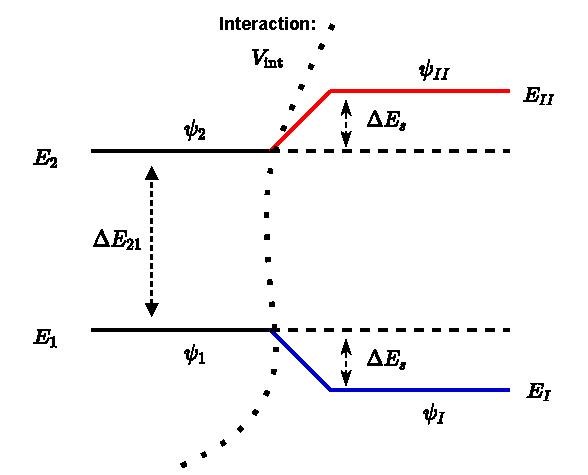
\includegraphics[width=0.7\textwidth]{Chapters/Figures/two-state-mixing.pdf}
    \caption{Defining the mixing between two different states, with two corresponding energies and wave-functions. Interaction is illustrated via the curved line and $V_\text{int}$ term.}
    \label{two-state-mixing-scheme}
\end{figure}

The problem consists of finding the final energies and wave-functions, this being done via the diagonalization procedure of a $2\times 2$ matrix. The main diagonal of this matrix contains the two energies and the off-diagonal terms represent the interaction itself. The final states will be denoted with ($E_I$, $E_{II}$) for the energies and ($\psi_I$, $\psi_{II}$) for the wave-functions. As a general rule, the mixing depends on the initial separation $\Delta E_{21}=(E_2-E_1)$ and the matrix element $\bra{\psi_1}V_\text{int}\ket{\psi_2}$. For a large spacing the effect of a given matrix element will be quenched. Moreover, even a small matrix element can introduce a large mixing if the energy separation between the states is negligible (that is, the unperturbed states lie close to each other). 

A reduction from these two parameters can be performed, obtaining a general mixing expression that is valid for any arbitrary interaction and any initial spacing. As a first step, one should define the ratio between the spacing of the unperturbed states ($\Delta E_{21}$) and the strength of the matrix element:
\begin{align}
    R=\frac{\Delta E_{21}}{V_\text{int}}\ .
\end{align}
With this quantity, the newly perturbed energies $E_I$ and $E_{II}$ become \cite{casten2000nuclear}:
\begin{align}
    E_I&=\frac{1}{2}(E_1+E_2)+\frac{\Delta E_{21}}{2}\sqrt{1+\frac{4V_\text{int}^2}{\Delta E_{21}^2}}\ ,\\
    E_{II}&=\frac{1}{2}(E_1+E_2)-\frac{\Delta E_{21}}{2}\sqrt{1+\frac{4V_\text{int}^2}{\Delta E_{21}^2}}\ .
    \label{eq-two-state-mixing-energies}
\end{align}

Additionally, the amount by which each energy is shifted after the interaction is denoted in Fig. \ref{two-state-mixing-scheme} by $\Delta E_S$, and its expression depends on $\Delta E_{12}$ as:
\begin{align}
    |\Delta E_S|=|E_{II}-E_2|=|E_{I}-E_1|=\frac{\Delta E_{21}}{2}\left[\sqrt{1+\frac{4}{R^2}}-1\right]\ .
    \label{eq-shift-mixed-states}
\end{align}

The two perturbed wave functions are as follows:
\begin{align}
    \psi_I&=\alpha\psi_1+\beta\psi_2\ ,\nonumber\\
    \psi_{II}&=-\beta\psi_1+\alpha\psi_2\ ,
\end{align}
where the two amplitudes $\alpha$ and $\beta$ must verify the condition $\alpha^2+\beta^2=1$ and:
\begin{align}
    \beta=\frac{1}{\left\{1+\left[\frac{R}{2}+\sqrt{\frac{R^2}{4}+1}\right]^2\right\}^{1/2}}
    \label{eq-beta-mixing-amplitude}
\end{align}

It is noteworthy that the amplitude $\beta$ is in fact a function that only depends on $R$ (i.e., the ratio between the unperturbed energy splitting and the interaction strength). Similarly, by dividing the shift in energy $\Delta E_S$ to the initial splitting $\Delta E_{21}$, one will obtain an expression that is independent of the initial level spacing:
\begin{align}
    \frac{|\Delta E_S|}{\Delta E_{21}}=\frac{|E_{II}-E_{2}|}{\Delta E_{21}}=\frac{|E_{I}-E_{1}|}{\Delta E_{21}}=\frac{1}{2}\left[\sqrt{1+\frac{4}{R^2}}-1\right]
\end{align}

The importance of these formula will be now emphasized through a numerical example. Firstly, the evolution of the ratio of the unperturbed shift and the interaction can be graphically represented as functions of the small mixing amplitude $\beta$ though Eq. \ref{eq-beta-mixing-amplitude}. The obtained result is shown in Fig. \ref{fig-beta-mixing-amplitude}. Following this analysis, the shape of $R$ as a function of the energy shift of the perturbed states can be visualized in Fig. \ref{fig-beta-mixing-amplitude}.
\begin{figure}
    \centering
    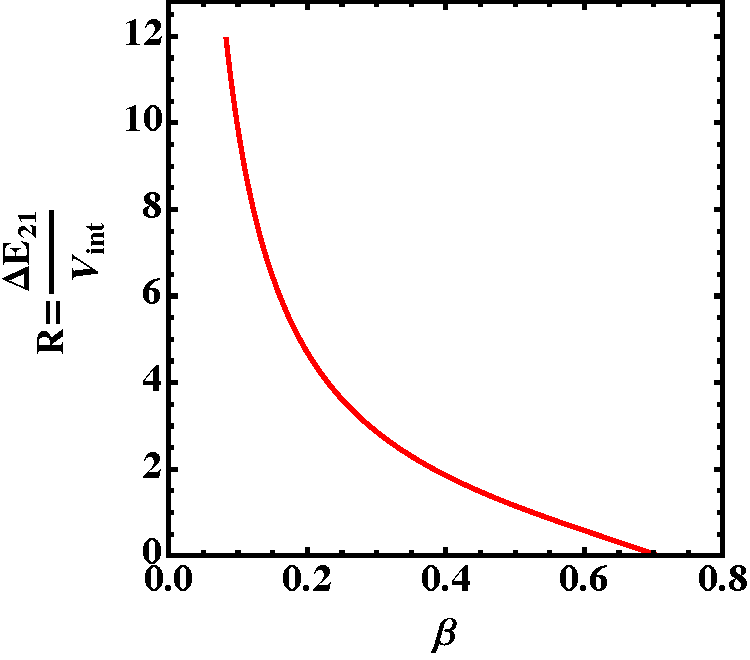
\includegraphics[width=0.5\textwidth]{Chapters/Figures/beta_mixing_amplitude.pdf}
    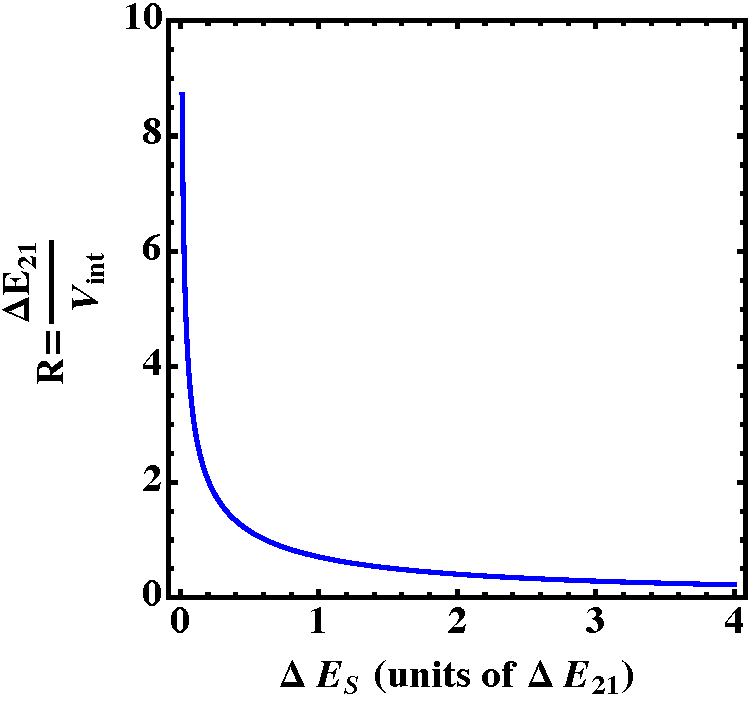
\includegraphics[width=0.49\textwidth]{Chapters/Figures/energy_shift_mixing_shape.pdf}
    \caption{\textbf{Left:} The dependence of $R$ on the mixing amplitude $\beta$. \textbf{Right}: The dependence of $R$ on the energy shift of the perturbed states ($\Delta E_S$).}
    \label{fig-beta-mixing-amplitude}
\end{figure}

For an arbitrary case where two initial states are separated by, say $\Delta_{21}=0.07$ MeV, and they become \emph{perturbed} via the interaction with a strength $V_\text{int}=0.03$ MeV, this gives a value of $R=3.5$ and a mixing amplitude of $beta=0.256$. The two states be both shifted by $\Delta E_S=5.31$ keV (accounting for about $7.6 \%$ of the initial separation). Indeed, for this particular example, the perturbation results in an energy shift that is rather small compared to the initial state spacing.

Besides the numerical example discussed above, there are also two other important limiting situations when the states interact via a perturbation. The first one is the so-called \emph{strong mixing limit}, when the initial states are degenerate (i.e., there is practically no spacing between them and $\Delta_{21}=0$). In this situation, the analytical expressions from Eq. \ref{eq-shift-mixed-states} fail to provide a quantitative analysis, but from Eq. \ref{eq-two-state-mixing-energies} a small adjustment can be made:
\begin{align}
    E_{I,II}=\frac{1}{2}\left[(E_1+E_2)\pm2V_\text{int}\right]=E_0\pm V_\text{int}\ ,
\end{align}
where the initial (common) energy of the degenerate states is denoted by $E_0$. The above equation indicates that the energy shift is only given by the \emph{mixing matrix element}. This means that the final separation energy for a two-state isolated system can never be closer than twice the interaction strength ($2V_\text{int}$). In the degeneracy case, the values for $\beta$ and $\alpha$ are readily obtained: ($\beta=\alpha=1/\sqrt{2}=0.707$), such that the states are completely mixed. Consequently, the mixed wave-functions of two (initially) degenerate states do not depend on the strength $V_\text{int}$. The limiting case of \emph{strong mixing} is sketched in Fig. \ref{strong-mixing-fig}.
\begin{figure}
    \centering
    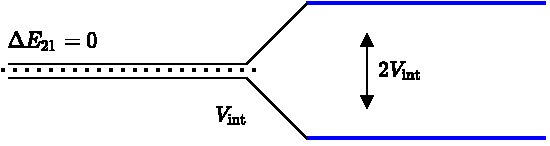
\includegraphics[scale=0.95]{Chapters/Figures/mixing_strong_coupling.pdf}
    \caption{The \emph{strong mixing} limit for two energy levels that are interacting via a perturbation. The initial two levels are degenerate, such that their splitting is null.}
    \label{strong-mixing-fig}
\end{figure}

The second limiting case is called \emph{weak mixing limit}, corresponding to a very large value of $R$ (meaning that the initial separation of the states is very large compared to the magnitude of the interaction itself). The shift in energy of the perturbed states in this case is given by:
\begin{align}
    \frac{|\Delta E_S|}{\Delta E_{21}}=\frac{1}{R^2}\ ,
\end{align}
and a graphical representation for weak mixing is shown in Fig. \ref{weak-mixing-fig}. 

As a final step in the analysis of two-state mixing, it is worth mentioning a corner-case that will help to get a better grasp of the Nilsson orbitals from Chapter \ref{chapter-2-theoretical-aspects} (recall Section \ref{subsection-nilsson-model}). Consider two states (say $\psi_1$ and $\psi_2$) whose energies are parametrized in terms of some argument $c_\text{nuc}$ relevant for the nuclear structure of that system (e.g., $c_\text{nuc}$ could be the quadrupole deformation and the two initial states are in fact Nilsson orbits). If there indeed exists mixing between the two states, \emph{they can never cross each other}. The two mixed states will always repel and they can never be closer than twice the mixing matrix element $V_\text{int}$ after mixing occurs. In Fig. \ref{fig-non-crossing} the behavior of non-crossing for the mixed states is sketched. The point at which the two states are the closest to each other represents the case when the wave-functions contain similar admixtures of each of the initial states (unperturbed). The \emph{inflection point} can be seen in Fig. \ref{fig-non-crossing}.
\begin{figure}
    \centering
    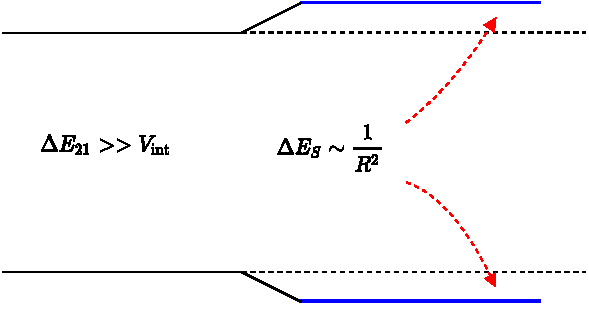
\includegraphics[scale=0.95]{Chapters/Figures/mixing_weak_coupling.pdf}
    \caption{The \emph{weak mixing} limit for two energy levels that are interacting via a perturbation. The interaction strength is much smaller than the initial spacing between states, resulting in a very small energy splitting $\Delta E_{S}$.}
    \label{weak-mixing-fig}
\end{figure}
\begin{figure}
    \centering
    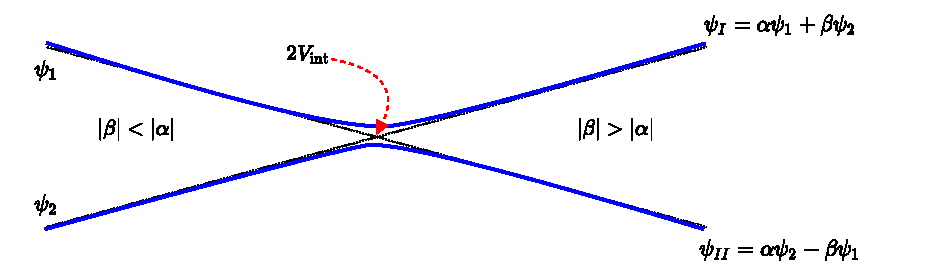
\includegraphics[scale=0.9]{Chapters/Figures/state_non_crossing.pdf}
    \caption{The \emph{non-crossing} between two states. The arrow marks the closest point at which the two states can interact with each other (i.e., the inflection point).}
    \label{fig-non-crossing}
\end{figure}
